%! Author = jesco
%! Date = 16.10.26
\section{Datensatzübersicht}
\label{sec:datensatzuebersicht}
Gegeben sind zwei XES-Dateien: InternationDeclarations.xes und DomesticDeclarations.xes, die je ein mit OpenXES generiertes konformes Log mit mehreren Traces und darunter Events enthalten.
Der Log-Untersuchungszeitraum liegt zwischen dem \todo{Datum} und dem \todo{Datum}.
% ------------------------------------------------------------------
% Basisstatistik (direkt aus den XES-Dateien ausgelesen, 14.10.2026)
% ------------------------------------------------------------------
\begin{table}[htbp]
\centering
\caption{Basisstatistik der Event-Logs}
\label{tab:basisstatistik}
\begin{tabular*}{\textwidth}{@{\extracolsep{\fill}} l c c @{}}
\hline
\textbf{Kennzahl} & \textbf{Domestic} & \textbf{International} \\ \hline
Cases & 10.500 & 6.449 \\
Events & 56.437 & 72.151 \\
Aktivitäten & 17 & 34 \\
Varianten (Celonis) & 100 & 756 \\
Case-Start 2016 / 2017 / 2018 & -- / 2.240 / 8.260 & 3 / 1.494 / 4.952 \\
Ressourcen (\texttt{org:resource}) & STAFF MEMBER, SYSTEM & STAFF MEMBER, SYSTEM \\ \hline
\end{tabular*}
\end{table}
InternationalDeclarations.xes enthält 6.449 Traces mit insgesamt 72.151 Events, während DomesticDeclarations.xes 10.500 Traces mit insgesamt 56.437 Events enthält.
\subsection{Trace-Attribute}
Die Traces in beiden Dateien enthalten Metadaten wie die 'id', 'concept:name', 'BudgetNumber', 'DeclarationNumber' und 'Amount'.
International enthält zusätzlich noch weitere Felder zu Permit, Travel oder Beträgen (Amounts).
Auffällig ist, dass grundsätzlich alle Felder an jedem Trace der jeweiligen Datei Werte beinhalten, jedoch auch der Wert 'UNKNOWN' verwendet wird.
\begin{figure}
    \centering
    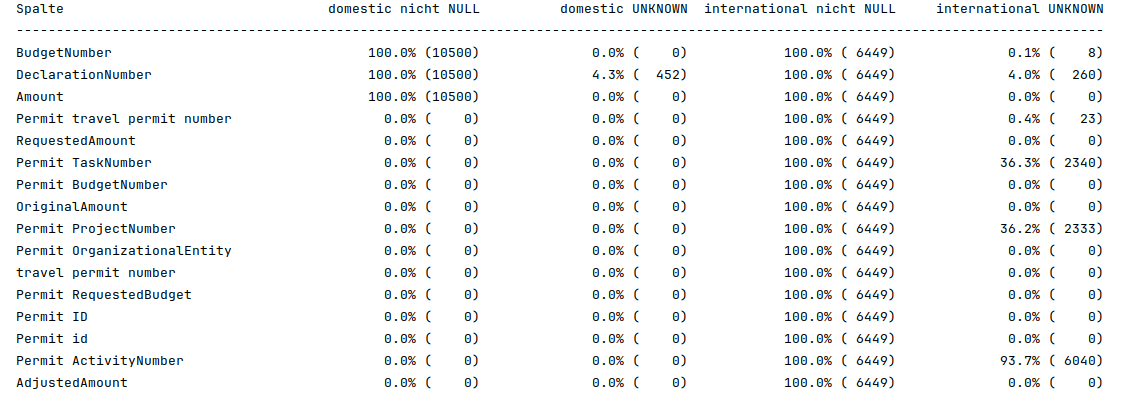
\includegraphics[width=\textwidth]{figures/python/attribute}
    \caption{}
\end{figure}
\begin{wrapfigure}{r}{0.45\textwidth}
    \centering
    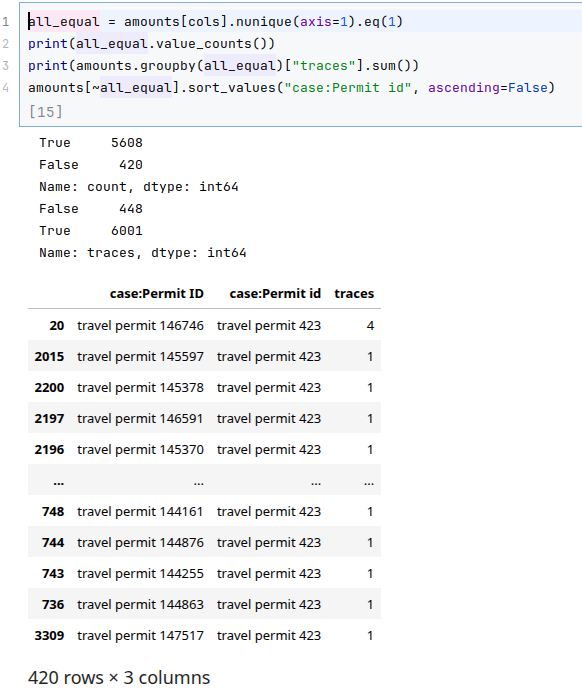
\includegraphics[width=0.45\textwidth]{figures/python/permitid}
    \caption{}
    \label{fig:permitid}
\end{wrapfigure}
Zudem gibt es in der Vielzahl der Eigenattribute von International semantische Ähnlichkeiten, die untersucht wurden.
'Permit ID' und 'Permit id' unterscheiden sich nur in der Groß-/Kleinschreibung.
Bei der Betrachtung der enthaltenen Werte, zeigt sich, dass überwiegend diese übereinstimmen, allerdings 448 Fälle existieren, in denen 'Permit id' abweichend von 'Permit ID' den Wert 'travel permit 423' enthält.
Der Wert 'travel permit 423' ist dabei nicht nur für den Fall relevant, sondern wird auch für einen Trace mit 'Permit ID' = 'travel permit 423' verwendet, wo damit eine Übereinstimmung vorliegt.
Auf eine mögliche Erklärung dieser 448/449 Fälle wird in Kapitel \todo{Kapitellink} eingegangen.
Auch die Amount-Felder 'Amount' / 'RequestedAmount' / 'AdjustedAmount' / 'OriginalAmount' wurden zusammen untersucht und zusätzlich mit 'Permit RequestedBudget' gegenübergestellt.
Es konnte festgestellt werden dass in 6448 von 6449 Fällen die ersteren 4 Felder den gleichen Wert enthalten bei 6001 verschiedenen Wertkombinationen, während zu RequestedBudget nur 24 Traces eine Gleichheit gefunden werden konnte, davon 21 Fälle mit dem Amount 0.
'case:Permit travel permit number' und 'case:travel permit number' sind in 5970 Fällen identisch und weichen in 479 Fällen voneinander ab.
'case:id' und 'case:concept:name' sind in beiden Logs je Trace immer identisch und eindeutig.
\begin{table}[htbp]
    \centering
    \caption{Attribute und Anzahl distinkter Werte je Log}
    \label{tab:attribut-maechtigkeiten}
    \footnotesize
    \setstretch{1}
    \renewcommand{\arraystretch}{1.15}
    \begin{tabularx}{\textwidth}{@{}p{2cm}XX@{}}
        \toprule
        & \textbf{Domestic (10.500 Traces)} & \textbf{International (6.449 Traces)} \\
        \midrule
        Gemeinsame Attribute
        & \texttt{id}: 56.437\par
          \texttt{org:resource}: 2\par
          \texttt{concept:name}: 17\par
          \texttt{time:timestamp}: 45.403\par
          \texttt{org:role}: 7\par
          \texttt{case:id}: 10.500\par
          \texttt{case:concept:name}: 10.500\par
          \texttt{case:BudgetNumber}: 1\par
          \texttt{case:DeclarationNumber}: 10.049\par
          \texttt{case:Amount}: 8.326
        & \texttt{id}: 69.073\par
          \texttt{org:resource}: 2\par
          \texttt{concept:name}: 34\par
          \texttt{time:timestamp}: 51.270\par
          \texttt{org:role}: 8\par
          \texttt{case:id}: 6.449\par
          \texttt{case:concept:name}: 6.449\par
          \texttt{case:BudgetNumber}: 719\par
          \texttt{case:DeclarationNumber}: 6.190\par
          \texttt{case:Amount}: 6.100 \\
        \midrule
        Log-spezifische Attribute
        & /
        & \texttt{case:Permit travel permit number}: 5.596\par
          \texttt{case:RequestedAmount}: 6.100\par
          \texttt{case:Permit TaskNumber}: 6\par
          \texttt{case:Permit BudgetNumber}: 207\par
          \texttt{case:OriginalAmount}: 6.100\par
          \texttt{case:Permit ProjectNumber}: 825\par
          \texttt{case:Permit OrganizationalEntity}: 27\par
          \texttt{case:travel permit number}: 6.033\par
          \texttt{case:Permit RequestedBudget}: 5.259\par
          \texttt{case:Permit ID}: 6.028\par
          \texttt{case:Permit id}: 5.608\par
          \texttt{case:Permit ActivityNumber}: 145\par
          \texttt{case:AdjustedAmount}: 6.101 \\
        \bottomrule
    \end{tabularx}
\end{table}

\subsection{Event-Daten}
In beiden Logs enthält ein Event die gleichen 5 Attribute: 'id', 'org:resource', 'concept:name', 'time:timestamp' und 'org:role'.
'id' und 'time:timestamp' sind Metadaten zu dem betroffenen Event.
'concept:name' beschreibt die durchgeführte Aktivität.
'org:resource' erklärt den Ursprung des Events, ob SYSTEM oder STAFF MEMBER, während 'org:role' die Rolle des Event-Akteurs wiedergibt.
Jedem möglichen Wert von 'concept:name' ist eine eindeutige Kombination aus 'org:resource' und 'org:role' zugeordnet.
\begin{figure}
    \centering
    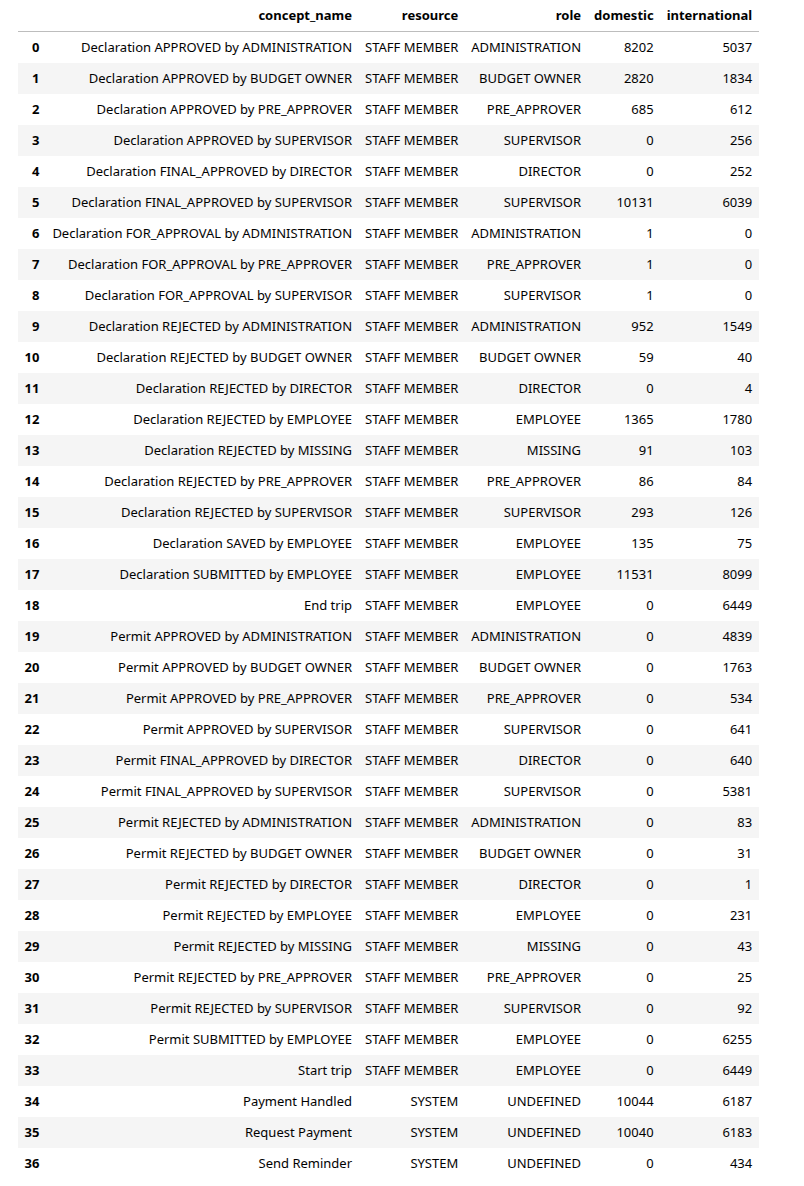
\includegraphics[width=0.7\linewidth]{figures/python/eventtypes}
    \caption{}
    \label{fig:eventtypes}
\end{figure}
Bei Domestic sind alle im Log enthaltenen Events in ihrer id eindeutig, während bei International einzelne Events (Kennung über id und time:timestamp) mehrfach vorkommen.
Dies betrifft 1480 Event-Ids mit insgesamt 4558 Nennungen.
Eine Abweichung des Timestamps oder des concept:name innerhalb der gleichen Event-Id gibt es bei allen Nennungen in dem Log nicht, weswegen von dem selben Event ausgegangen werden kann.
Mit einer Differenz von 3078 ($4558-1480$) IDs wird der Unterschied der initialen 72.151 Events (Tabelle \ref{tab:basisstatistik}) zu den 69.073 distinkten Event-Ids in \todo{\ref{tab:attribut-maechtigkeiten}} erklärt.
